\chapter{THỬ NGHIỆM VÀ PHƯƠNG PHÁP ĐÁNH GIÁ}\label{ch:kiemthu}

\section{Cơ sở đánh giá và cấu hình thử nghiệm}
Các phép thử được tổ chức riêng cho từng khối phần cứng, từng thuật toán xử lý và từng chặng truyền thông. Sau đó, hệ thống được đối chiếu tổng thể trên toàn bộ chuỗi từ thiết bị đeo đến giao diện giám sát. Mỗi phép thử đều xác định rõ cấu hình, điều kiện thực hiện, dữ liệu cần ghi nhận và công thức tính toán chỉ tiêu để đảm bảo khả năng lặp lại và so sánh khách quan.

Riêng đối với trạm chuyển tiếp Gateway sử dụng Raspberry Pi 3 Model B kết hợp mô-đun SIM 4G, nội dung đánh giá tập trung vào khả năng tiếp nhận gói RF, chuyển tiếp bản tin MQTT, lưu đệm dữ liệu khi mất mạng và tự động khôi phục kết nối. Các chỉ tiêu về độ trễ truyền dẫn, tỷ lệ mất gói và độ ổn định được tổng hợp từ nhật ký thực nghiệm. Các phép tính lý thuyết được trình bày độc lập và phân biệt rõ với số liệu đo đạc thực tế.

Mỗi phiên thử nghiệm bắt buộc phải ghi nhận các thông tin định danh gồm mã người tham gia, vị trí gắn thiết bị, dải đo cảm biến, tần số lấy mẫu, phiên bản mô hình, cấu hình RF, thông số modem và phiên bản phần mềm Gateway. Việc thử nghiệm trên một cá nhân hay một vị trí lắp đặt duy nhất chưa đủ cơ sở để kết luận về năng lực tổng quát hóa của thuật toán nhận dạng hoạt động. Tương tự, việc thử nghiệm thiết bị đặt tĩnh trên bàn không thể thay thế cho đánh giá thực tế khi thiết bị được cố định chắc chắn trên cơ thể người lính và vận hành đồng bộ cùng toàn bộ phần cứng.

\section{Kiểm thử khối phần cứng và lấy mẫu dữ liệu}\label{sec:testhardware}
\subsection{Kiểm tra trạng thái phần cứng trước khi tích hợp}
Quy trình kiểm tra phần cứng bắt đầu bằng việc đo đạc nguồn điện không tải và có tải, kiểm tra thứ tự cấp nguồn, mức điện áp logic trên bus và độ chắc chắn của các đầu nối cơ khí. Tiếp theo, hệ thống đọc mã định danh các vi mạch IC, xác nhận địa chỉ I\textsuperscript{2}C của cảm biến và kiểm tra chiều trục không gian bằng các tư thế xoay góc đã biết trước. Ở trạng thái đứng yên, kỹ thuật viên quan sát giá trị bias của con quay hồi chuyển, độ lớn gia tốc và từ trường; khi quay từng trục, cần kiểm tra chiều tăng giảm tương ứng của tín hiệu. Các bước kiểm tra này giúp khoanh vùng và tách biệt lỗi lắp đặt phần cứng khỏi lỗi thuật toán phần mềm.

Trong quá trình tích hợp toàn hệ thống, các phép kiểm tra trên cần được lặp lại trong các trạng thái vận hành đồng thời gồm phát sóng RF, kết nối BLE, modem 4G hoạt động và cảm biến khí được cấp nguồn nhiệt. Hệ thống ghi nhận các sự kiện khởi động lại của ESP32 hoặc Raspberry Pi, số mẫu cảm biến bị lỗi, tình trạng treo bus giao tiếp và biên độ dao động nguồn. Nếu một sự cố chỉ xuất hiện khi tải công suất vô tuyến tăng cao, kỹ thuật viên phải ưu tiên kiểm tra chất lượng nguồn cấp và bố trí mạch trước khi tiến hành điều chỉnh bộ lọc tín hiệu.

\begingroup\SmallTable
\begin{longtable}{|P{40bp}|P{155bp}|P{213bp}|}
\caption{Kịch bản kiểm thử các khối phần cứng hệ thống}\label{tab:hwtest}\\\hline
\textbf{Mã}&\textbf{Nội dung kịch bản thử nghiệm}&\textbf{Dữ liệu và dấu hiệu cần ghi nhận}\\\hline\endfirsthead
\hline\textbf{Mã}&\textbf{Nội dung kịch bản thử nghiệm}&\textbf{Dữ liệu và dấu hiệu cần ghi nhận}\\\hline\endhead
HW01&Kiểm tra bật nguồn lặp lại&Điện áp nguồn, mã nguyên nhân reset, thời gian khởi tạo cảm biến và lỗi nhận diện vi mạch IC.\\\hline
HW02&Đánh giá trạng thái đứng yên&Giá trị trung bình gyro, độ trôi theo thời gian, độ lớn gia tốc và nhiệt độ bo mạch.\\\hline
HW03&Kiểm tra quay góc chuẩn&Chiều trục, dấu góc xoay, sai số tại từng tư thế và hiện tượng qua ranh giới $0^\circ/360^\circ$.\\\hline
HW04&Phát sóng RF và kết nối modem&Độ sụt áp nguồn, hiện tượng reset, lỗi giao tiếp I\textsuperscript{2}C, số mẫu thiếu và nhiễu hướng từ.\\\hline
HW05&Lắp hoàn chỉnh pin và vỏ hộp&Sự thay đổi từ trường so với bo rời; sai số do vỏ, ốc vít, dây dẫn và độ rơ cơ khí.\\\hline
HW06&Ngắt quãng hoặc tháo cảm biến&Thời gian phát hiện lỗi, cờ báo dữ liệu không hợp lệ và khả năng tự khôi phục của chương trình.\\\hline
\end{longtable}\endgroup

\subsection{Đánh giá chất lượng lấy mẫu thời gian thực}
Giả sử các dấu thời gian liên tiếp của mẫu dữ liệu được ghi nhận là $t_i$, chu kỳ lấy mẫu thực tế giữa hai mẫu là $\Delta t_i = t_i - t_{i-1}$. Tần số lấy mẫu trung bình $\hat{f}_s$ trong một phiên ghi nhận được tính toán theo biểu thức:
\begin{equation}
\hat f_s=\frac{N-1}{t_N-t_1}.
\end{equation}
Bên cạnh giá trị trung bình, báo cáo cần thống kê chi tiết sự phân bố của $\Delta t_i$, khoảng gián đoạn thời gian lớn nhất và số lượng mẫu bị mất. Nếu hoạt động truyền thông vô tuyến làm thay đổi chu kỳ lấy mẫu, người thu mẫu bắt buộc phải điều chỉnh lại lịch tác vụ hoặc dung lượng bộ đệm trước khi sử dụng tập dữ liệu đó cho việc huấn luyện hoặc suy luận.

\section{Đánh giá phân hệ nhận dạng hành động}
\subsection{Thiết kế và thu thập dữ liệu kiểm tra}
Dữ liệu kiểm tra phải bao gồm đầy đủ các hoạt động mục tiêu, các giai đoạn chuyển tiếp tư thế giữa những hành động khác nhau và các tình huống dễ gây nhầm lẫn. Mỗi tình nguyện viên thực hiện nhiều phiên đo tách biệt; nhãn nhịp thời gian được đối chiếu chính xác qua quan sát trực tiếp hoặc video ghi hình. Các động tác té ngã chỉ được phép mô phỏng trong điều kiện an toàn có kiểm soát nhằm giảm thiểu tối đa nguy cơ chấn thương cho người tham gia.

Tập dữ liệu kiểm tra phải được tách biệt hoàn toàn khỏi tập huấn luyện theo đối tượng người dùng hoặc theo phiên đo trước khi tiến hành cắt cửa sổ trượt. Nếu hai cửa sổ dữ liệu có nội dung gần như trùng lặp bị chia đều sang cả hai tập, chỉ số đánh giá độ chính xác sẽ bị tăng giả tạo dù mô hình chưa có khả năng tổng quát hóa tốt.

\subsection{Các chỉ tiêu đánh giá và thời gian đáp ứng hệ thống}
Đối với mỗi lớp hành động $c$, các chỉ tiêu đánh giá được tính toán dựa trên số lượng dự đoán đúng ($TP_c$), dự đoán nhầm ($FP_c$) và bỏ sót ($FN_c$):
\begin{align}
\mathrm{Precision}_c&=\frac{TP_c}{TP_c+FP_c}, &
\mathrm{Recall}_c&=\frac{TP_c}{TP_c+FN_c},\\
F1_c&=\frac{2\,\mathrm{Precision}_c\,\mathrm{Recall}_c}{\mathrm{Precision}_c+\mathrm{Recall}_c}.
\end{align}
Mọi trường hợp mẫu số bằng không đều phải được xử lý theo quy ước công bố rõ ràng. Báo cáo cần trình bày ma trận nhầm lẫn, tổng số mẫu của từng lớp và chỉ số trung bình macro-F1 nhằm tránh việc các lớp có nhiều dữ liệu che khuất chất lượng của các lớp ít dữ liệu. Riêng đối với lớp hành động ngã, hệ thống cần quan sát kỹ tỷ lệ bỏ sót và tỷ lệ báo động giả theo thời gian, không chỉ dựa vào độ chính xác tổng thể.

Tổng thời gian đáp ứng của hệ thống bao gồm thời gian chờ đầy cửa sổ dữ liệu, thời gian trích xuất đặc trưng, thời gian suy luận trên vi điều khiển, thời gian truyền qua BLE và RF, thời gian xử lý tại Gateway, và thời gian cập nhật lên giao diện.

\section{Đánh giá hướng di chuyển, bước chân và quỹ đạo}\label{sec:testpdr}
\subsection{Thử nghiệm hướng đứng yên và quay góc có kiểm soát}
Cố định thiết bị đeo ở tư thế lắp đặt chuẩn, ghi nhận giá trị góc hướng trong khoảng thời gian đứng yên, sau đó lặp lại phép đo khi đã đóng vỏ, lắp pin và kích hoạt toàn bộ các khối phát vô tuyến. Người thực hiện tiến hành quay người qua các mốc góc chuẩn theo cả hai chiều, đặc biệt lưu ý kiểm tra khả năng xử lý qua ranh giới chuyển góc $359^\circ \rightarrow 0^\circ$. Phép thử này giúp phát hiện độ lệch bias của con quay hồi chuyển, lỗi ngược chiều trục, sai sót chuẩn hóa góc và mức độ ảnh hưởng nhiễu từ phần cứng.

Sai số góc được tính toán thông qua khoảng cách ngắn nhất trên vòng tròn lượng giác:
\begin{equation}
e_{\psi,i}=\operatorname{atan2}\!\left[\sin(\hat\psi_i-\psi_i^{ref}),\cos(\hat\psi_i-\psi_i^{ref})\right].
\end{equation}
Các giá trị góc trong biểu thức đều tính bằng đơn vị radian. Cách tính này giúp tránh tình trạng tính sai lệch giữa $359^\circ$ và $1^\circ$ thành $358^\circ$. Kết quả thực nghiệm cần được phân nhóm theo điều kiện từ trường thay vì gộp chung mọi phép thử thành một giá trị trung bình duy nhất.

\subsection{Thử nghiệm bước chân, quãng đường và đường đi khép kín}
Các tuyến đường thử nghiệm bao gồm đoạn đi thẳng, đổi hướng tại các góc vuông chuẩn, quay lại điểm xuất phát và di chuyển theo vòng khép kín. Mỗi tuyến đường được thực hiện ở nhiều dải tốc độ khác nhau; kỹ thuật viên ghi lại số bước tham chiếu, chiều dài thực tế, vị trí các điểm rẽ và mốc thời gian tương ứng. Nếu thay đổi vị trí gá lắp hoặc chiều gắn bo mạch, dữ liệu đó phải được ghi nhận như một điều kiện thử nghiệm hoàn toàn mới.

Sai số bước chân tương đối và sai số điểm cuối hành trình được xác định theo công thức:
\begin{align}
e_N&=\frac{|\hat N-N^{ref}|}{N^{ref}}\,100\%,\\
e_{end}&=\sqrt{(\hat x_{end}-x_{end}^{ref})^2+(\hat y_{end}-y_{end}^{ref})^2}.
\end{align}
Đối với các mốc tham chiếu dọc tuyến đường, hệ thống có thể tính toán thêm chỉ số sai số quân phương (RMSE) về vị trí. Sai số điểm cuối của tuyến đường khép kín chỉ phản ánh một phần hiện tượng trôi tích lũy chứ không mô tả toàn bộ sai số tại từng đoạn ngắn; do đó cần lưu trữ đồng thời quỹ đạo kèm mốc thời gian thay vì chỉ ghi nhận tọa độ điểm dừng cuối cùng.

\subsection{Phân tích định lượng ảnh hưởng của sai số hướng}
Để đánh giá độ nhạy của thuật toán PDR, ta khảo sát một đoạn đường thẳng dài $L$ có sai lệch góc hướng không đổi $\delta\psi$. Thành phần sai lệch ngang $e_\perp$ được xác định theo hệ thức hình học:
\begin{equation}
e_{\perp}=L\,|\sin\delta\psi|.
\end{equation}
Hình~\ref{fig:drift} và Bảng~\ref{tab:drift} thể hiện kết quả tính toán mô phỏng từ công thức trên, hoàn toàn không phải số liệu đo đạc thực tế của thiết bị đeo. Phân tích này chỉ nhằm cô lập ảnh hưởng của sai số hướng; trong hệ thống thực tế còn tồn tại thêm sai số phát hiện bước chân, sai số chiều dài bước và sự biến động hướng ngẫu nhiên theo thời gian.

\begin{figure}[htbp]\centering\begin{tikzpicture}
\begin{axis}[width=.94\linewidth,height=7cm,
xlabel={Quãng đường thẳng $L$ (m)},ylabel={Sai lệch ngang $e_{\perp}$ (m)},
xmin=0,xmax=30,ymin=0,ymax=3,xtick={0,5,...,30},ytick={0,.5,...,3},
grid=both,major grid style={black!20},minor grid style={black!8},
tick label style={font=\fontsize{11bp}{13bp}\selectfont},
label style={font=\fontsize{12bp}{14bp}\selectfont},
legend style={at={(.5,-.26)},anchor=north,legend columns=3,font=\fontsize{11bp}{13bp}\selectfont,draw=none},
every axis plot/.append style={line width=.8pt}]
\addplot[black,domain=0:30,samples=2]{x*sin(1)};\addlegendentry{$\delta\psi=1^\circ$}
\addplot[black,dashed,domain=0:30,samples=2]{x*sin(3)};\addlegendentry{$\delta\psi=3^\circ$}
\addplot[black,dashdotted,domain=0:30,samples=2]{x*sin(5)};\addlegendentry{$\delta\psi=5^\circ$}
\end{axis}
\end{tikzpicture}

\caption{Sai lệch ngang tính toán lý thuyết khi góc hướng bị lệch một góc không đổi}
\label{fig:drift}\end{figure}

\begingroup\SmallTable
\begin{table}[htbp]\centering
\caption{Ví dụ tính toán sai lệch ngang theo quãng đường di chuyển (đơn vị: mét)}\label{tab:drift}
\begin{tabular}{|c|c|c|c|}\hline
Quãng đường $L$ & $\delta\psi = 1^\circ$ & $\delta\psi = 3^\circ$ & $\delta\psi = 5^\circ$ \\\hline
10 & 0,17 & 0,52 & 0,87 \\\hline
20 & 0,35 & 1,05 & 1,74 \\\hline
30 & 0,52 & 1,57 & 2,61 \\\hline
\end{tabular}\end{table}\endgroup

Như vậy, một sai lệch hướng nhỏ chỉ $5^\circ$ trên đoạn đường thẳng 30 m đã tạo ra khoảng 2,61 m sai lệch ngang ngay cả khi chiều dài bước chân được tính toán hoàn toàn chính xác. Do đó, các giải pháp thuần túy làm mượt đường vẽ trên giao diện hay tăng tần suất truyền dữ liệu không thể giải quyết được tận gốc lỗi sai lệch hướng. Mọi cải tiến thuật toán đều phải được kiểm chứng thực nghiệm trên cùng tuyến đường chuẩn để xác định chính xác phần sai số được giảm thiểu thực tế.

\section{Kiểm thử đường truyền RF, trạm Gateway và mạng 4G}\label{sec:testgateway}
\subsection{Đo đạc tỷ lệ mất gói, độ trễ và tuổi dữ liệu}
Mỗi gói tin phát đi từ thiết bị đeo đều được đánh số thứ tự tuần tự; bộ thu RF, trạm Gateway và dịch vụ máy chủ ghi lại đồng thời kèm theo mã định danh thiết bị. Tỷ lệ chuyển giao gói tin thành công ở một chặng được tính trên tổng số gói tin duy nhất nhận được so với số gói đã phát:
\begin{equation}
\mathrm{PDR}_{pkt}=\frac{N_{nhan,duy\ nhat}}{N_{gui}}\,100\%.
\end{equation}
Các gói tin bị lặp được thống kê độc lập và không cộng vào số gói thành công. Kỹ thuật viên cần phân biệt rõ hiện tượng mất kết nối RF với tình trạng gói tin đã lưu trong hàng đợi đệm nhưng chưa đến được Broker do mạng 4G bị gián đoạn. Các yếu tố như khoảng cách tới Gateway, vật cản kiến trúc, tư thế cơ thể, vị trí đặt ăng-ten và tổng số thiết bị hoạt động đồng thời đều phải được ghi lại như các điều kiện thử nghiệm cố định.

Độ trễ truyền dẫn một chiều chỉ có ý nghĩa khi các đồng hồ thời gian trên thiết bị đã được đồng bộ chính xác hoặc có phương pháp ước lượng sai lệch độ trễ. Trường hợp không đảm bảo điều kiện đồng bộ thời gian tuyệt đối, hệ thống sử dụng phương pháp đo vòng khứ hồi hoặc khoảng thời gian xử lý trên cùng một máy chủ. Tuổi dữ liệu hiển thị trên giao diện người dùng cũng cần được đo đạc riêng biệt vì có thể chịu ảnh hưởng bởi chu kỳ cập nhật của màn hình đồ họa.

\subsection{Kịch bản mô phỏng mất kết nối và khả năng tự khôi phục}
\begingroup\SmallTable
\begin{longtable}{|P{39bp}|P{150bp}|P{219bp}|}
\caption{Danh mục kịch bản kiểm thử trạm Gateway và đường truyền thông}\label{tab:nettest}\\\hline
\textbf{Mã}&\textbf{Tình huống sự cố mô phỏng}&\textbf{Điều kiện nghiệm thu yêu cầu chức năng}\\\hline\endfirsthead
\hline\textbf{Mã}&\textbf{Tình huống sự cố mô phỏng}&\textbf{Điều kiện nghiệm thu yêu cầu chức năng}\\\hline\endhead
NET01&Mất kết nối BLE giữa bộ đeo và mũ&Nút trên mũ phát hiện mất dữ liệu bộ đeo; tuyệt đối không sử dụng giá trị cũ như số đo mới.\\\hline
NET02&Mất kết nối RF về trạm Gateway&Trạm Gateway tăng chỉ số tuổi dữ liệu, hiển thị trạng thái mất kết nối nút; không tự sinh tọa độ giả.\\\hline
NET03&Ngắt kết nối mạng 4G của Gateway&Trạm Gateway lưu giữ các gói tin hợp lệ vào hàng đợi bền vững theo đúng chính sách dung lượng.\\\hline
NET04&Khôi phục kết nối mạng 4G&Gateway tiến hành gửi dữ liệu bù kèm dấu thời gian gốc; cơ chế chống trùng lặp hoạt động chính xác; giao diện phân biệt rõ dữ liệu lịch sử.\\\hline
NET05&Khởi động lại máy chủ Pi 3B&Kiểm tra hàng đợi lưu đệm còn nguyên vẹn dữ liệu, khóa phiên hoạt động và cơ chế tự khởi động lại dịch vụ.\\\hline
NET06&MQTT Broker từ chối kết nối&Ghi nhận mã lỗi xác thực hoặc lỗi mạng; tuyệt đối không xóa bỏ các gói tin chưa được chuyển giao thành công.\\\hline
NET07&Nhiều nút mạng gửi đồng thời&Đo đạc hiện tượng tranh chấp kênh, tỷ lệ mất gói, thời gian phục hồi và mức độ đầy của hàng đợi Gateway.\\\hline
\end{longtable}\endgroup

Trạng thái tự phục hồi kết nối phải được đánh giá đồng thời trên cả phần mềm Gateway và ứng dụng giám sát. Việc biểu tượng kết nối chuyển sang màu xanh không thể thay thế cho việc đối chiếu dữ liệu đến đủ, không trùng lặp và đúng thứ tự thời gian. Tương tự, một lần xuất bản MQTT thành công chưa đủ để chứng minh toàn bộ nguồn cấp, mô-đun SIM và dịch vụ mạng hoạt động ổn định trong thời gian dài.


\subsection{Ghi nhận dữ liệu MQTT bằng công cụ MQTTX}\label{subsec:mqttx-minhchung}
Để kiểm tra khả năng tiếp nhận bản tin ở tầng ứng dụng, công cụ MQTTX được sử dụng đăng ký chủ đề \nolinkurl{ssalab/firefighter1} trên MQTT Broker. Hình~\ref{fig:mqttx-minhchung} là ảnh chụp phiên làm việc cho thấy MQTTX đã nhận một bản tin có cấu trúc JSON. Các trường quan sát được gồm \texttt{rawAct}, \texttt{hmmAct}, \texttt{stepCount}, \texttt{stepDistance}, \texttt{directionValue}, \texttt{directionHeading}, cùng các tập mẫu \texttt{positionSamples} và \texttt{inertialSamples}. Nhóm mẫu quán tính bao gồm dữ liệu gia tốc và vận tốc góc theo ba trục; các trường vị trí phục vụ kiểm tra đầu ra của thuật toán PDR.

\begin{figure}[htbp]
  \centering
  \IfFileExists{assets/mqttx-nhan-du-lieu.png}{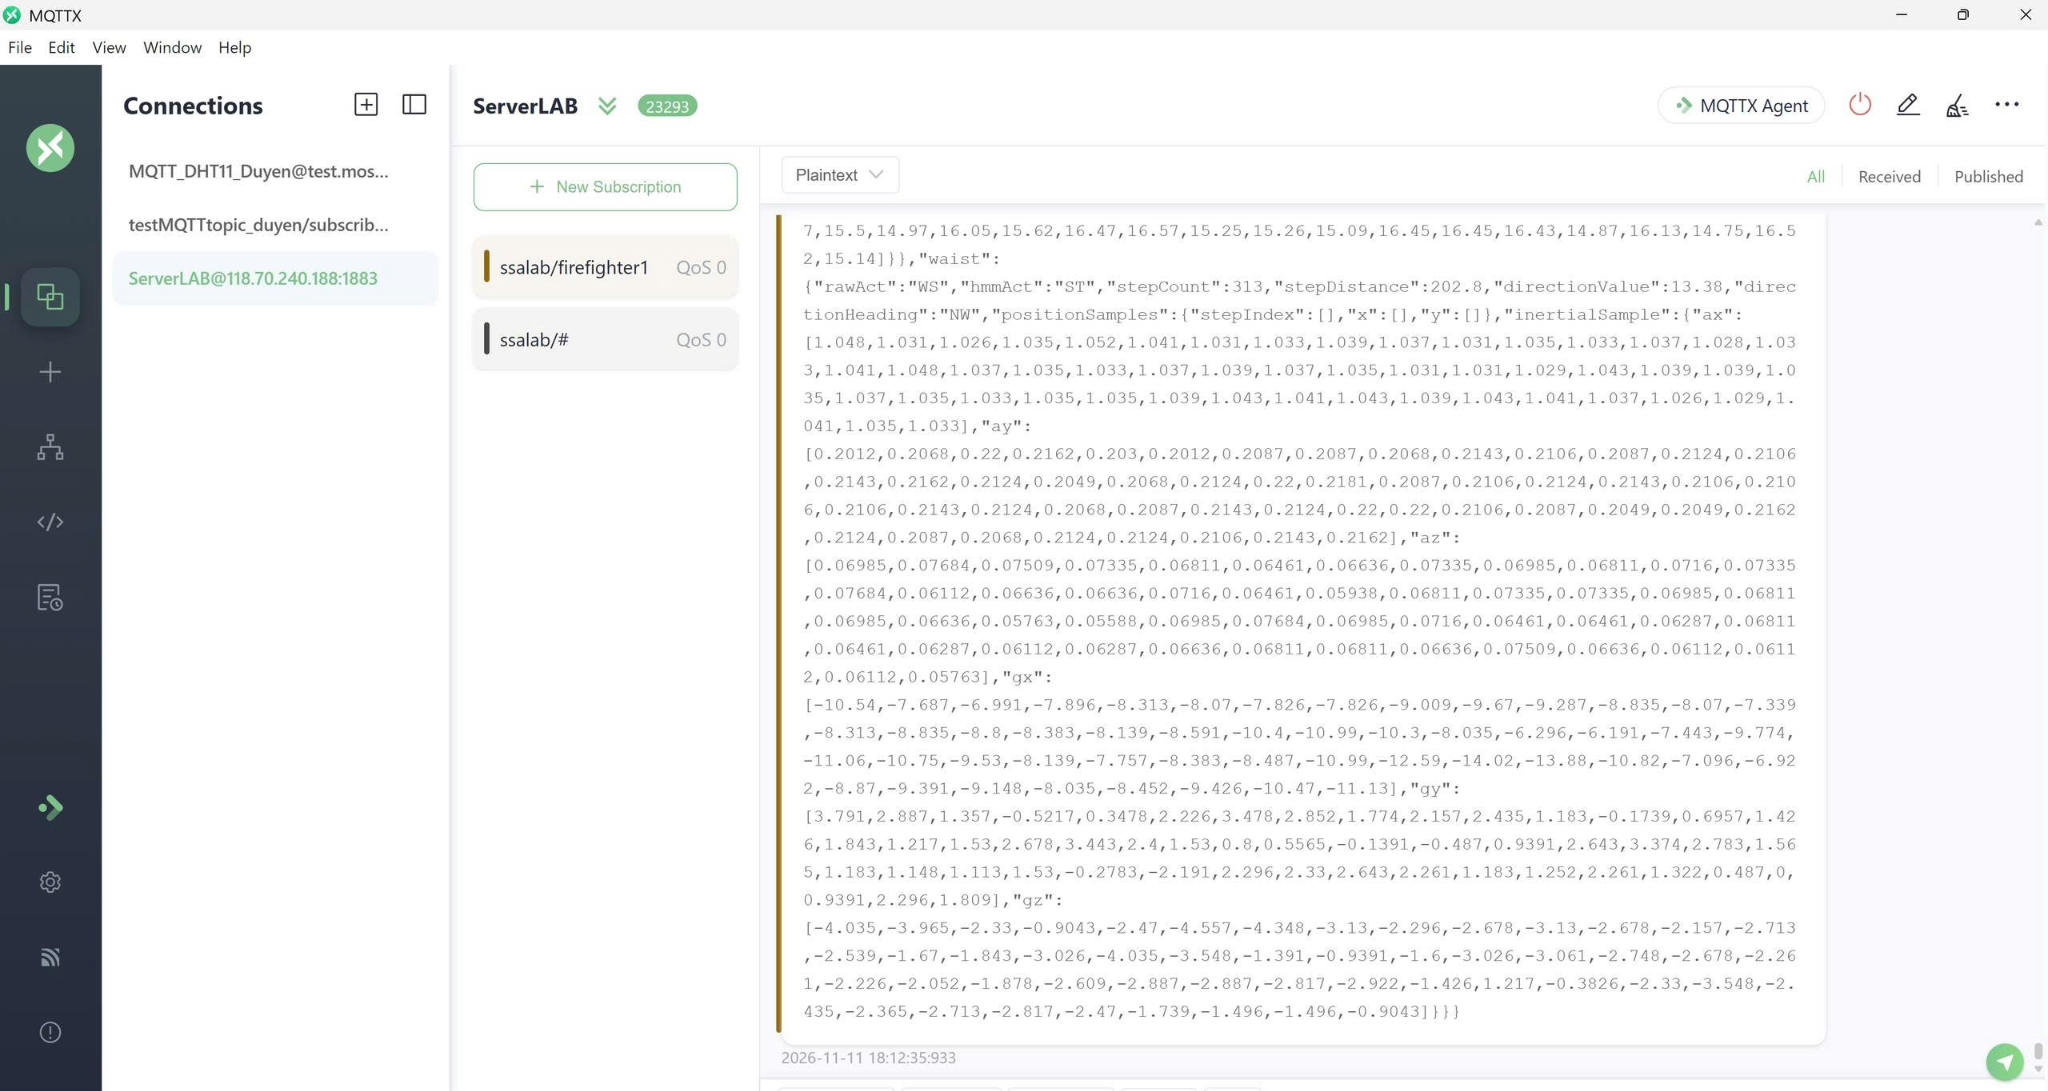
\includegraphics[width=\linewidth,height=.58\textheight,keepaspectratio]{assets/mqttx-nhan-du-lieu.png}}{\fbox{\parbox{.82\linewidth}{Ảnh MQTTX tiếp nhận bản tin JSON được cung cấp trong gói tư liệu bổ sung.}}}
  \caption{Ảnh chụp MQTTX nhận bản tin JSON trên chủ đề giám sát thiết bị}
  \label{fig:mqttx-minhchung}
\end{figure}

Tại thời điểm chụp, bản tin hiển thị \texttt{stepCount} bằng 313 và \texttt{stepDistance} bằng 202,8, minh họa việc đồng thời truyền trạng thái vận động, dữ liệu bước chân và các chuỗi mẫu cảm biến trong một thông điệp. Ảnh chụp chỉ xác nhận dữ liệu xuất hiện tại phía MQTT client trong phiên kiểm tra; chưa đủ để định lượng tỷ lệ mất gói, độ trễ đầu cuối hoặc xác minh riêng chặng RF 433 MHz và 4G. Các chỉ tiêu này vẫn cần được đánh giá bằng kịch bản đo kiểm độc lập đã nêu ở trên.

\section{Kiểm tra đáp ứng dữ liệu khí độc và áp suất khí quyển}
Các cảm biến khí MQ-9 và MQ-135 có đặc tính vật lý phụ thuộc rất lớn vào loại khí, điều kiện môi trường làm việc và quy trình hiệu chuẩn thực tế. Cảm biến MQ-135 là linh kiện bán dẫn nhạy cảm với nhiều nhóm khí khác nhau và khói tổng hợp; do đó dữ liệu của nó không thể tự tương đương với một chỉ số chất lượng không khí chuẩn (AQI) hay một phép đo khí CO\textsubscript{2} chọn lọc~\cite{mq135}. Tài liệu kỹ thuật của từng phiên bản MQ-9/MQ-9B phải được đối chiếu cẩn thận khi thiết kế mạch gia nhiệt và xây dựng phương pháp khai thác tín hiệu~\cite{mq9}.

Trước khi thiết lập được quy trình hiệu chuẩn chuẩn hóa với khí tham chiếu, dữ liệu thu nhận từ cảm biến khí nên được lưu trữ dưới dạng giá trị tín hiệu thô (ADC) hoặc tỷ số đặc trưng, đi kèm trạng thái làm nóng và cờ báo hợp lệ. Các con số biểu diễn PPM hiển thị trên giao diện chỉ mang tính chất minh họa giao diện, tuyệt đối không được sử dụng như số liệu đo đạc đã qua kiểm định. Hơn nữa, mô hình hiện tại không trực tiếp đo lường nồng độ khí oxy, do đó không được suy diễn điều kiện đủ oxy trong không khí chỉ dựa vào tín hiệu từ MQ-9 hay MQ-135.

Đối với cảm biến áp suất BMP580, các phép thử cần thực hiện tại các mốc cao độ cố định đã biết, duy trì khoảng thời gian ổn định đủ để cảm biến và vỏ hộp đạt trạng thái cân bằng nhiệt - áp. Kỹ thuật viên cần ghi nhận lại trạng thái cửa phòng, hệ thống thông gió và nhiệt độ bo mạch trong suốt quá trình đo. Nếu mục tiêu đặt ra là hỗ trợ phân loại tầng lầu, hệ thống cần xác định rõ điểm áp suất tham chiếu $p_0$, cao độ thực tế của các tầng, điều kiện chuyển tầng và quy tắc nhận biết khi dữ liệu áp suất không còn đáng tin cậy.